% !TEX program = xelatex
% !TEX encoding = UTF-8
\documentclass[a4paper,10pt,twocolumn]{ctexart}

%% ========== Page Layout ==========
\usepackage[top=1.7cm, bottom=1.8cm, left=1.7cm, right=1.7cm, columnsep=0.7cm]{geometry}

%% ========== Fonts (CVPR-style: Times + 宋体/黑体) ==========
\usepackage{fontspec}
\setmainfont{Times New Roman}
\usepackage{xeCJK}
\setCJKmainfont[AutoFakeBold=2.2, AutoFakeSlant=0.15]{SimSun}            % 中文正文：宋体
\setCJKsansfont[AutoFakeBold=2.5]{SimHei}            % 无衬线（标题等）：黑体
\setCJKmonofont{SimSun}
\setCJKfamilyfont{hei}[AutoFakeBold=2.5]{SimHei}
\newcommand{\hei}{\CJKfamily{hei}}
% 中西文边界间距固定为很小的可压缩值，避免两栏窄列里被过度拉伸出大空隙
\xeCJKsetup{CJKecglue={\hskip 0.08em plus 0.02em minus 0.04em}}

%% ========== Headers & Footers ==========
\usepackage{fancyhdr}
\pagestyle{fancy}
\fancyhf{}
\fancyhead[L]{\small\itshape AdaIN StyleKV：基于自注意力KV融合与自适应归一化的扩散模型免训练风格迁移}
\fancyhead[R]{\small\thepage}
\fancyfoot{}
\renewcommand{\headrulewidth}{0.4pt}
\setlength{\headheight}{14pt}

%% ========== Spacing ==========
\linespread{1.05}
\setlength{\parindent}{1.8em}
\setlength{\parskip}{1pt plus 1pt minus 1pt}
\setlength{\abovedisplayskip}{5pt plus 2pt minus 2pt}
\setlength{\belowdisplayskip}{5pt plus 2pt minus 2pt}
% 两栏窄列断行更宽容，减少行内被拉开的大空隙
\tolerance=2000
\emergencystretch=3em
\hyphenpenalty=1000
% 浮动体放置参数：允许大图（尤其跨栏 figure*）更积极地占据页面顶部
\renewcommand{\topfraction}{0.95}
\renewcommand{\bottomfraction}{0.95}
\renewcommand{\textfraction}{0.05}
\renewcommand{\floatpagefraction}{0.7}
\renewcommand{\dbltopfraction}{0.95}
\renewcommand{\dblfloatpagefraction}{0.7}
\setcounter{topnumber}{3}
\setcounter{dbltopnumber}{3}
\setcounter{totalnumber}{5}

%% ========== Tables & Figures ==========
\usepackage{booktabs}
\usepackage{multirow}
\usepackage{array}
\usepackage{graphicx}
\usepackage{caption}
\usepackage{placeins}
\usepackage{float}
\captionsetup{labelsep=period, labelfont={small,bf}, textfont={small}}
\captionsetup[table]{skip=4pt}
\captionsetup[figure]{skip=4pt}

%% ========== Math & Symbols ==========
\usepackage{amsmath,amssymb}
\newcommand{\cmark}{$\checkmark$}
\newcommand{\xmark}{$\times$}

%% ========== Section Titles (CVPR-style) ==========
\usepackage{titlesec}
\titleformat{\section}{\normalfont\large\sffamily\bfseries}{\thesection.}{0.6em}{}
\titleformat{\subsection}{\normalfont\normalsize\sffamily\bfseries}{\thesubsection.}{0.6em}{}
\titleformat{\subsubsection}{\normalfont\normalsize\sffamily\bfseries}{\thesubsubsection.}{0.6em}{}
\titlespacing*{\section}{0pt}{2.0ex plus 0.5ex minus 0.2ex}{1.0ex plus 0.2ex}
\titlespacing*{\subsection}{0pt}{1.6ex plus 0.4ex minus 0.2ex}{0.8ex plus 0.2ex}
\titlespacing*{\subsubsection}{0pt}{1.4ex plus 0.3ex minus 0.2ex}{0.6ex plus 0.2ex}

%% ========== Hyperlinks ==========
\usepackage[hidelinks]{hyperref}

%% ========== Title Formatting ==========
\usepackage{titling}
\setlength{\droptitle}{-2.6cm}

\graphicspath{{figures/}}

\begin{document}

% ===== Title block + teaser + abstract (CVPR-style, spanning full width) =====
\twocolumn[{%
\enlargethispage{4\baselineskip}
\begin{center}
  {\sffamily\bfseries\huge AdaIN StyleKV：基于自注意力KV融合与自适应归一化的\\[1pt]扩散模型免训练风格迁移}\\[4pt]
  {\normalsize 姜俊吉 \quad 吕卓靓 \quad 杨沛文}\\[1pt]
  {\normalsize 电子科技大学计算机（网安）学院}\\[1pt]
  {\normalsize \texttt{\{junji.jiang, zhuoliang.lv, peiwen.yang\}@uestc.edu.cn}}\\[4pt]
\end{center}

\begin{center}
  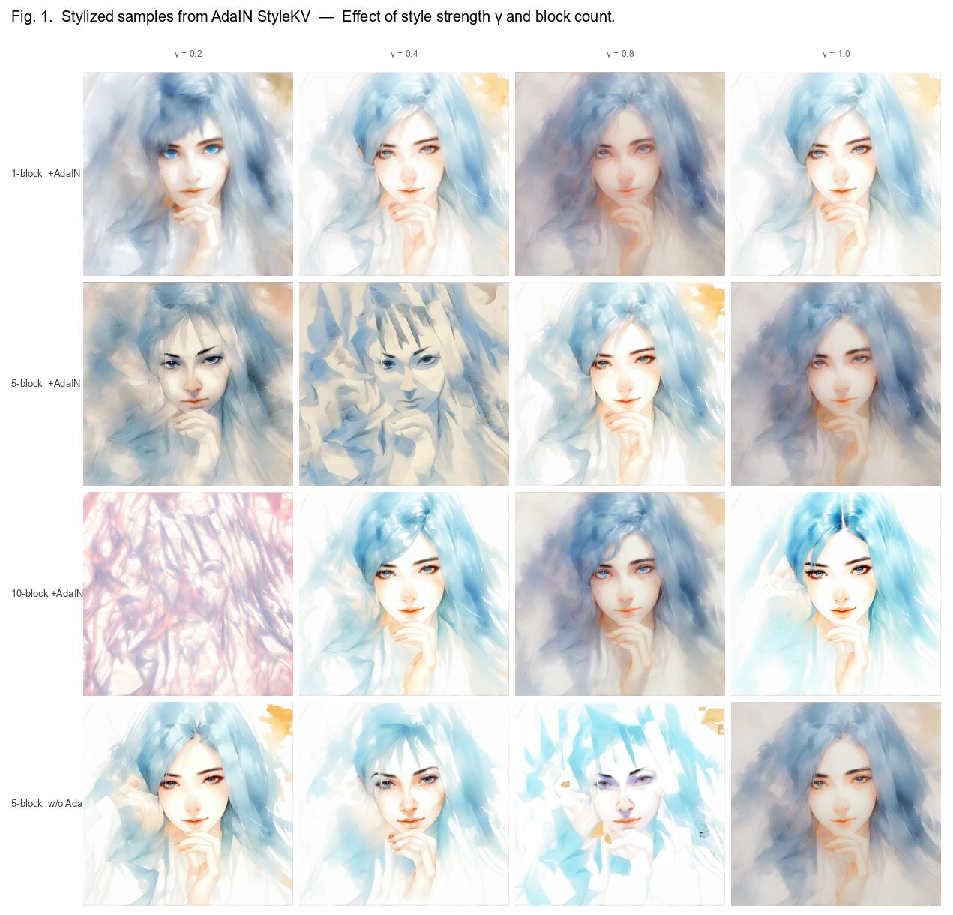
\includegraphics[width=0.82\textwidth]{fig_gallery.pdf}
  \captionof{figure}{AdaIN StyleKV风格迁移效果展示。图中展示了不同块数配置（1-block、5-block、10-block）和不同风格融合强度$\gamma$（0.2--1.0）下的生成结果。横向从左至右$\gamma$逐步增大，可清晰观察到风格纹理从弱到强的渐变过程；纵向从上至下分别为不同块数与AdaIN配置的组合。5-block +AdaIN 行（第二行）为本文完整方法，在$\gamma=0.6$附近达到风格强度与内容保真度的最佳平衡。}
  \label{fig:gallery}
\end{center}

\vspace{2pt}
\begin{minipage}{\textwidth}
\begin{center}{\sffamily\bfseries\normalsize 摘\quad 要}\end{center}
{\small\noindent 艺术风格迁移旨在将参考图像的视觉风格渲染到内容图像上，同时保留其语义结构。尽管扩散模型在该领域取得了显著进展，现有方法通常需要针对每种风格进行单独优化，或在大规模模型应用中难以在风格强度与内容保真度之间取得良好平衡。为此，本文提出 AdaIN StyleKV，一个构建于预训练扩散模型之上的免训练风格迁移框架。该方法集成了以下关键组件：(1) Canny ControlNet，用于在生成过程中保持内容图像的边缘与轮廓结构；(2) 选择性自注意力KV融合机制，受InstantStyle启发，仅在特定UNet解码器块中线性融合内容图像与风格图像的自注意力键值特征；(3) AdaIN自适应归一化模块，用于增强色彩风格迁移与氛围一致性。基于MS COCO内容数据集与WikiArt风格数据集的实验结果表明，本方法在ArtFID指标上达到85.43，在风格逼真度与内容保留度之间实现了较优平衡。此外，本文还实现了一个基于Gradio的交互式前端，支持用户实时调节风格强度、ControlNet参数及AdaIN融合系数。

\smallskip
\noindent{\sffamily\bfseries 关键词：}风格迁移；扩散模型；自注意力；自适应实例归一化；免训练；ControlNet}
\end{minipage}
\vspace{24pt}
}]

%% ================================================
%% 1. 引言
%% ================================================
\section{引言}

在计算机视觉与计算机图形学领域，图像艺术风格迁移一直是一个引人入胜的研究方向。给定一幅内容图像和一幅风格图像，风格迁移任务的目标是合成一幅输出图像，该图像既能保留原始场景的语义结构与空间布局，又能充分体现参考图像的视觉风格，包括纹理、笔触和色彩调色板等要素。

风格迁移的发展经历了从非参数化纹理合成[1]、基于优化的神经网络方法[2]、前馈卷积网络[3,4]到生成对抗网络（GAN）[5,6,7]的范式演进。每一种范式都带来了生成速度与迁移质量的显著提升，但同时也存在固有局限：GAN类方法通常局限于训练阶段所见过的风格域，难以泛化至任意风格；而基于优化的方法计算开销高昂，难以满足实时应用需求。

近年来，扩散模型（Diffusion Models）[8,9,10]的兴起极大地推动了生成建模领域的进展。Stable Diffusion[11]及其后续版本凭借潜在扩散机制与交叉注意力模块，能够从文本提示生成高分辨率、语义丰富的图像。受此启发，研究人员自然地将扩散模型扩展至风格迁移任务[12,13,14,15,16,17]。然而，现有基于扩散的方法仍面临若干显著挑战。首先，InST[12]和StyleDiffusion[13]等方法需要对每种新的风格图像进行基于梯度的微调或文本反演，单幅图像的风格适应往往耗时较长，限制了其在大规模或实时场景中的应用。其次，部分方法在应用于潜在扩散模型时难以可靠地保持原始图像的空间布局与语义结构，可能在迁移纹理的同时改变内容的几何形态。再者，自注意力操作虽然能够有效迁移局部纹理模式，但往往忽略全局颜色统计信息，导致输出图像在色调上缺乏整体协调性。此外，大多数现有方法缺少在风格强度与内容保真度之间进行灵活调节的机制，限制了用户的创作自由度。

针对上述挑战，本文提出AdaIN StyleKV——一个构建于预训练扩散模型之上的免训练风格迁移框架，无需任何微调或文本反演即可实现高质量的风格化。在结构保持方面，该框架引入Canny边缘检测引导的ControlNet，通过在生成过程中保留内容图像的边缘与轮廓结构，有效增强语义内容的稳定性。在纹理迁移方面，受InstantStyle[17]启发，我们设计了一种选择性自注意力KV融合策略，仅在特定的UNet解码器块中将内容图像的自注意力键和值特征与风格图像的对应特征进行线性融合，从而实现局部纹理模式的有效迁移。在色彩一致性方面，我们在特征层面引入自适应实例归一化（AdaIN）模块，通过对齐内容特征与风格特征的通道级均值和方差，增强色彩风格迁移与整体氛围的和谐统一。此外，该框架还通过引入融合系数$\gamma$，为用户提供了直观且连续的风格强度控制能力，使其能够在风格化程度与内容保留之间进行灵活取舍。

我们在MS COCO[18]内容数据集和WikiArt[19]风格数据集上对本文方法进行了系统的消融实验验证。定量评估涵盖ArtFID[20]、FID[21]和LPIPS[22]等多个维度。实验结果表明，AdaIN StyleKV在风格保真度与内容保留之间取得了较优平衡，以85.43的ArtFID值优于各消融变体。此外，我们还通过多组对比实验，系统揭示了不同配置（如KV融合块数量、融合系数$\gamma$、AdaIN模块的有无）对风格迁移效果的影响规律。为提升方法的实用性与可交互性，本文还实现了一个基于Gradio的交互式前端演示系统，支持用户实时调整风格强度、ControlNet参数和AdaIN融合系数。

%% ================================================
%% 2. 相关工作
%% ================================================
\section{相关工作}

\subsection{神经风格迁移}

神经风格迁移由Gatys等人[2]开创，他们使用VGG[23]特征的Gram矩阵匹配通过迭代优化实现风格迁移。后续工作主要聚焦于提升速度与泛化能力：Johnson等人[24]引入了基于感知损失的前馈图像变换网络，实现了实时风格迁移；Huang和Belongie[4]提出了自适应实例归一化（AdaIN），实现了前馈式的任意风格迁移。其他值得关注的方法包括基于注意力的方法[25,26,27]、基于流的方法[28]和对比学习框架[29]。尽管这些方法在速度上相比Gatys等人的优化式方法有显著提升，但在处理高度抽象或非写实风格时仍存在局限。

\subsection{基于GAN的风格迁移}

生成对抗网络在不成对图像翻译任务上取得了显著进展。CycleGAN[5]引入了循环一致性损失，使得无需配对数据即可实现跨域图像转换；StarGAN[6]进一步将其扩展为多领域转换框架，能够以单一模型处理多个目标域之间的翻译任务。此外，以StyleGAN[7]及其变体[30,31]为代表的高质量生成模型，提供了精细且可解释的潜在空间控制能力，被广泛用于领域内的图像编辑与属性操作。但需要指出的是，StyleGAN本质上是一个无条件生成模型，其设计目标并非跨域翻译；在应用于领域外风格迁移时，往往需要额外的微调或特征解耦策略，难以直接实现与CycleGAN等翻译方法等价的任意风格泛化。

\subsection{基于扩散模型的风格迁移}

扩散模型已成为高质量图像生成的主导范式。其中，潜在扩散模型（LDM）[11]通过将图像压缩至低维潜在空间，实现了高效的训练与推理。针对风格迁移任务，研究者基于扩散模型提出了多种方法：

InST[12]采用文本反演技术将风格图像嵌入至文本向量空间，能够较好地保留风格特征，但需要对每种风格单独进行优化。StyleDiffusion[13]引入基于CLIP的损失函数与微调策略，以实现内容与风格的解耦。DiffStyle[14]是一种运行于扩散模型H空间的免训练方法，然而将其应用于Stable Diffusion时可能会改变图像的语义布局。Style Injection[16]通过将自注意力层中的键值特征替换为风格图像的特征，实现了免训练的风格迁移并保留了内容结构，但其颜色迁移能力有限。InstantStyle[17]发现仅有特定的UNet块对风格迁移起关键作用，并通过对这些块进行特征嵌入实现了高效的风格注入。相关工作进一步提出了对指定块特征嵌入进行选择性改进的方法。

\begin{center}
\resizebox{\columnwidth}{!}{%
\begin{tabular}{lcccc}
  \toprule
  方法 & 免训练 & 结构保持 & 色彩迁移 & 强度可控 \\
  \midrule
  InST[12] & \xmark & \xmark & \cmark & \xmark \\
  StyleDiffusion[13] & \xmark & \xmark & \cmark & \cmark \\
  DiffStyle[14] & \cmark & \xmark & \xmark & \xmark \\
  Style Injection[16] & \cmark & \xmark & \xmark & \xmark \\
  InstantStyle[17] & \cmark & \xmark & \xmark & \xmark \\
  \textbf{AdaIN StyleKV (本文)} & \cmark & \cmark & \cmark & \cmark \\
  \bottomrule
\end{tabular}%
}
\captionof{table}{本文方法与代表性风格迁移方法的对比。免训练：无需梯度优化；结构保持：显式引入结构约束；色彩迁移：专门处理全局色彩信息。}
\label{tab:method_comparison}
\end{center}

表~\ref{tab:method_comparison}总结了本文方法与代表性方法的异同。本文方法直接建立在InstantStyle的块选择策略、Style Injection的KV替换思想以及ControlNet的结构控制基础之上。在此基础上，我们进一步引入了AdaIN模块与加权融合机制，从而在纹理迁移与色彩和谐之间取得了更好的平衡。

\subsection{扩散模型中的条件控制}

ControlNet[15]提出了一种神经架构，使用零卷积层向扩散模型添加空间条件控制（边缘、深度、姿态等）。它将原始模型锁定并创建一个可训练的副本，确保训练不会破坏预训练特征。本文集成ControlNet的Canny边缘版本，以在执行风格迁移的同时保持内容图像的结构轮廓。需要注意的是，本文基于Stable Diffusion基础模型进行实验，所使用的ControlNet需与基础模型版本匹配（SD1.5版本对应 \texttt{lllyasviel/control\_v11p\_sd15\_canny}；SDXL版本对应 \texttt{diffusers/controlnet-canny-sdxl-1.0}）。当前实验基于SD1.5架构，未来计划将整套方法迁移至SDXL。

%% ================================================
%% 3. 方法
%% ================================================
\section{方法}

本章详细阐述我们提出的AdaIN StyleKV方法。我们首先介绍整体框架，然后逐一讲解选择性KV融合、初始潜变量AdaIN、ControlNet集成等核心组件。

\subsection{整体框架}

我们的方法基于Stable Diffusion + ControlNet（Canny）+ IP-Adapter，并在此基础上提出AdaIN StyleKV改进。整体框架分为以下五个阶段：

\medskip
\noindent{\bfseries 阶段一：图像预处理与编码。} 给定内容图像和风格图像，我们首先提取内容图像的Canny边缘图，作为ControlNet的条件输入。然后，使用VAE编码器将内容图像、风格图像和Canny边缘图分别编码到潜空间。

\medskip
\noindent{\bfseries 阶段二：DDIM反演与特征缓存。} 我们使用DDIM采样器对内容图像和风格图像分别进行反演，得到它们在每个时间步的潜变量。在风格图像的反演过程中，我们缓存每个指定自注意力块中的键特征和值特征，供后续的内容生成过程使用。

\medskip
\noindent{\bfseries 阶段三：初始潜变量AdaIN调制。} 我们不直接将内容图像的反演结果作为生成起点，而是使用AdaIN对其与风格图像的初始噪声进行调制。调制后的初始噪声在保留内容空间结构的同时，融入了风格图像的色调统计信息。

\medskip
\noindent{\bfseries 阶段四：反向扩散与KV融合。} 从调制后的初始噪声开始执行反向扩散过程。在每个时间步：(1) 将当前潜变量输入U-Net，计算各层的查询、键、值特征；(2) 对于选定的目标自注意力块，将计算得到的K和V与之前缓存的风格K和V进行加权融合；(3) 使用融合后的K/V进行自注意力计算；(4) 对于非目标块，保持原始的K/V不变。

\medskip
\noindent{\bfseries 阶段五：解码与输出。} 反向扩散完成后，得到生成图像的潜变量。将其输入VAE解码器，得到最终的风格化图像。

\begin{figure}[htbp]
  \centering
  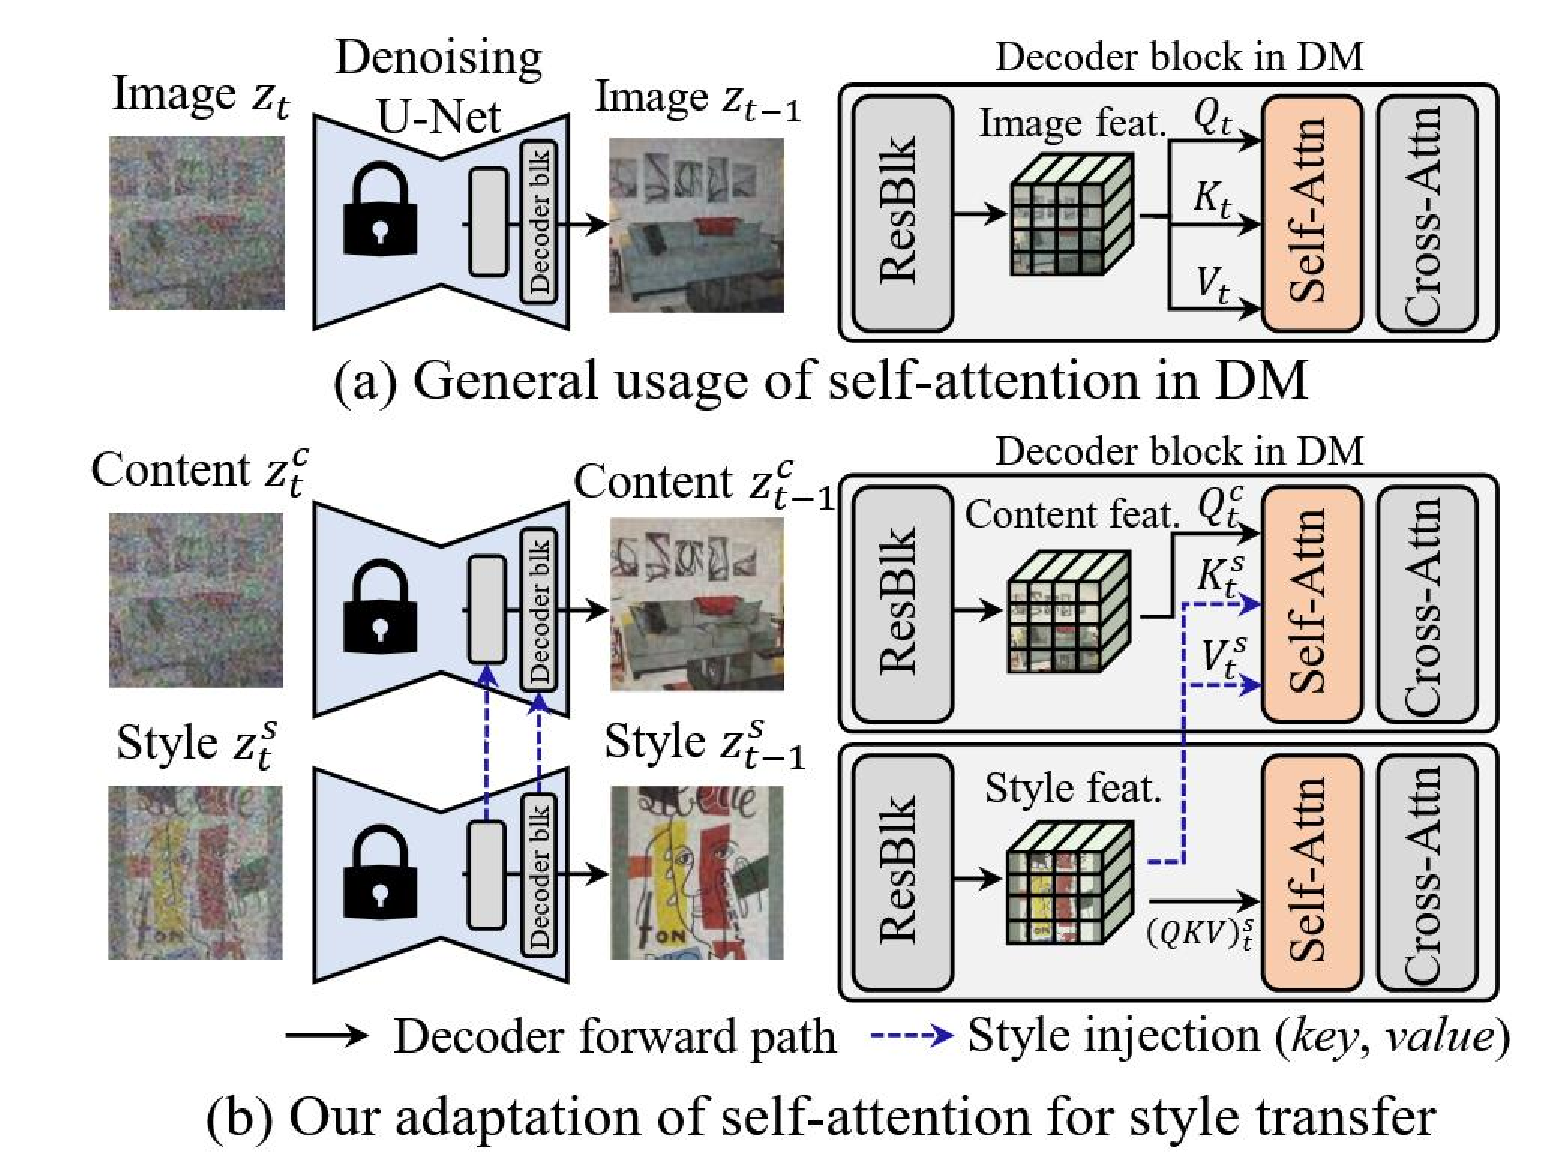
\includegraphics[width=\columnwidth]{fig_method_pipeline.pdf}
  \caption{AdaIN StyleKV整体方法流程框架图。给定内容图像与风格图像，首先通过Canny边缘检测提取内容结构信息，经VAE编码后进入潜空间；在DDIM反演阶段缓存风格图像特定UNet块的自注意力K/V特征；初始潜变量经AdaIN调制后作为反向扩散的起点；反向扩散过程中在选定块进行KV加权融合，最终经VAE解码器生成风格化图像。}
  \label{fig:pipeline}
\end{figure}

图~\ref{fig:pipeline}以可视化方式总结了上述五阶段流程，清晰展示了内容图像与风格图像在潜空间中的交互过程。

\subsection{选择性KV融合}

\subsubsection{自注意力机制回顾}

在U-Net中，自注意力层的计算方式如下。给定残差块输出的特征$X$，首先通过三个投影矩阵得到查询$Q$、键$K$和值$V$：
\begin{equation}
Q = X W_Q, \quad K = X W_K, \quad V = X W_V \label{eq:qkv}
\end{equation}
然后，通过缩放点积注意力计算输出：
\begin{equation}
\text{Attention}(Q, K, V) = \text{softmax}\!\left(\frac{QK^T}{\sqrt{d_k}}\right)V \label{eq:attention}
\end{equation}
其中$d_k$是查询向量的维度。在标准的生成过程中，$Q$、$K$、$V$都来自同一张图像的特征。但在风格迁移任务中，我们希望内容图像的结构（由$Q$主导）与风格图像的纹理（由$K$、$V$主导）相结合。

\begin{figure}[htbp]
  \centering
  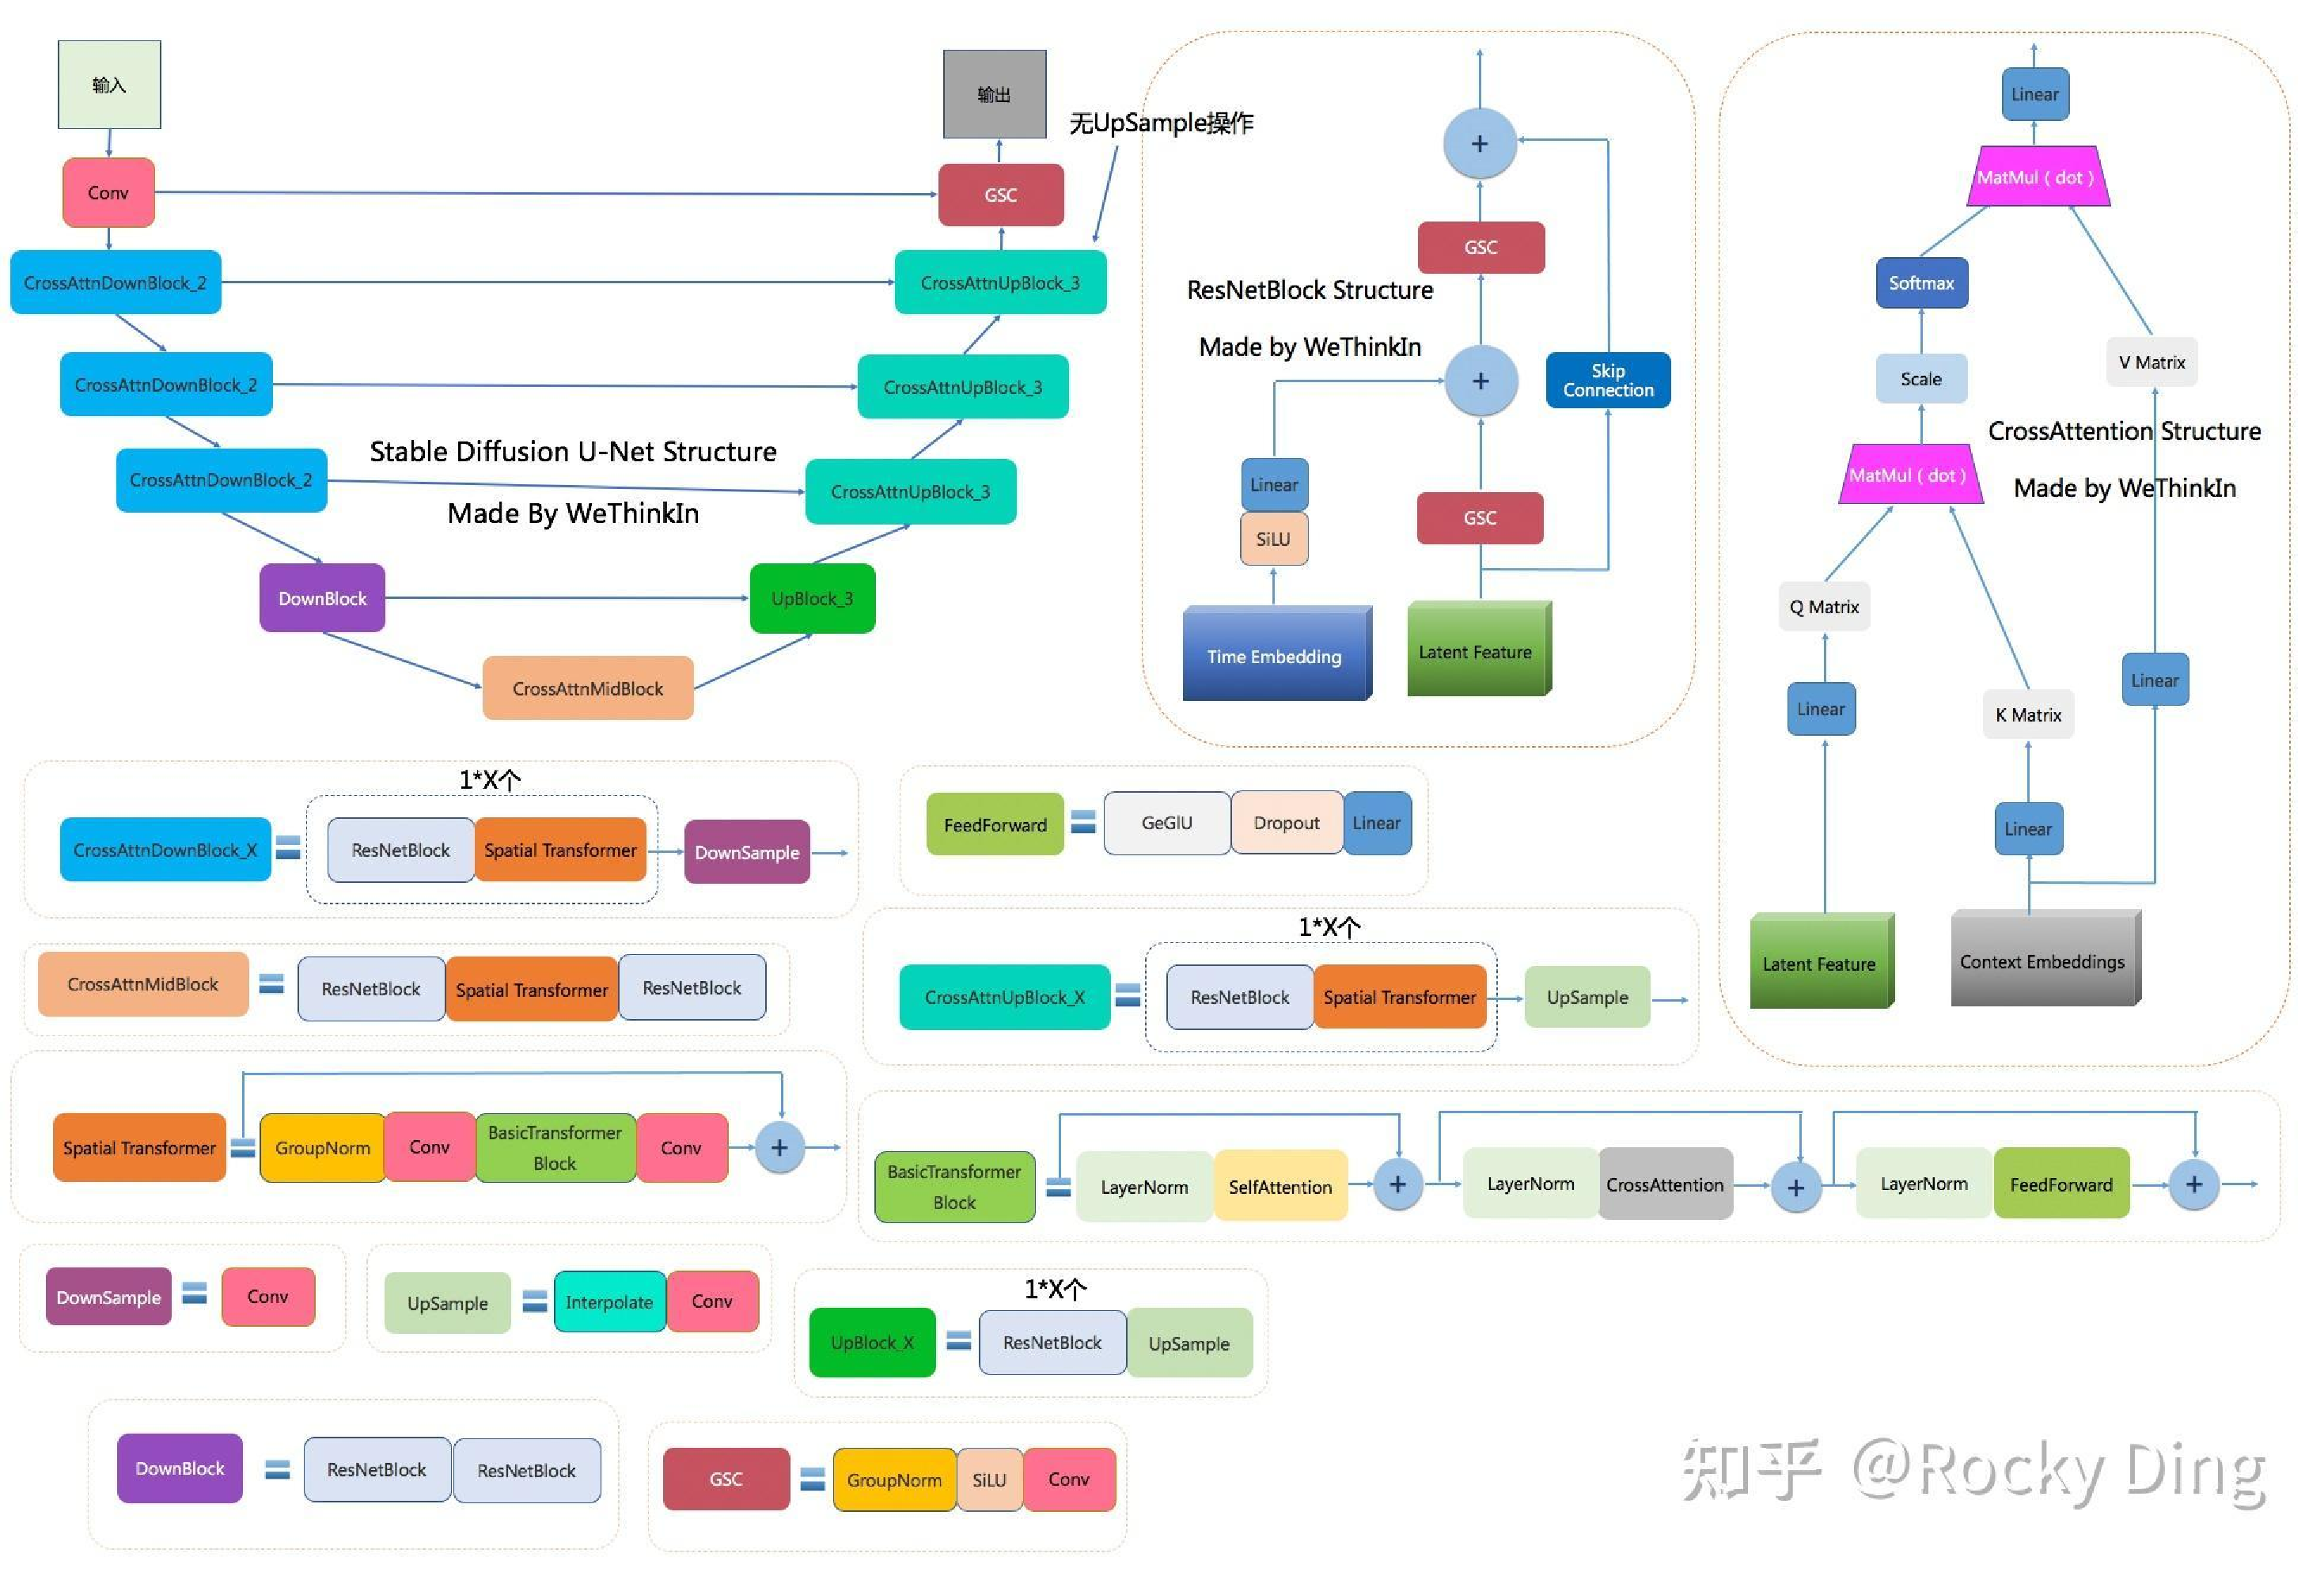
\includegraphics[width=\columnwidth]{fig_unet_arch.pdf}
  \caption{Stable Diffusion中U-Net架构示意图。U-Net由下采样编码器、中间块和上采样解码器三部分组成，每个部分包含多个ResNet残差块和自注意力层。本文方法仅在特定解码器块的自注意力层中进行KV融合（红色标记），其余块保持原有计算不变。}
  \label{fig:unet_arch}
\end{figure}

图~\ref{fig:unet_arch}展示了U-Net的整体架构及各层中自注意力模块的分布，为后续KV融合的目标块选择提供了结构参照。

\subsubsection{KV加权融合}

受到Style Injection[16]的启发，我们对选定自注意力块的K/V进行加权融合（而非直接替换）：
\begin{equation}
K_{\text{fused}} = (1 - \gamma) K_{\text{content}} + \gamma K_{\text{style}} \label{eq:kfusion}
\end{equation}
\begin{equation}
V_{\text{fused}} = (1 - \gamma) V_{\text{content}} + \gamma V_{\text{style}} \label{eq:vfusion}
\end{equation}
其中$\gamma \in [0, 1]$是风格融合强度系数。这种设计具有以下优势：(1) {\bfseries 可调节}：$\gamma=0$完全保留内容，$\gamma=1$完全使用风格，中间值平滑过渡；(2) {\bfseries 免训练}：仅通过线性插值实现风格注入，无需梯度优化；(3) {\bfseries 稳定性}：加权融合比直接替换更平滑，减少生成突变。

\subsubsection{目标块的选择}

遵循InstantStyle[17]的发现，我们不替换全部U-Net块，仅选择贡献最大的少数块。实验测试了三种配置：
\begin{itemize}
  \setlength{\itemsep}{0pt}
\item {\bfseries 1块}：仅替换 \texttt{up\_blocks.0.attentions.1}
\item {\bfseries 2块}：替换 \texttt{up\_blocks.0.attentions.1} 和 \texttt{down\_blocks.2.attentions.1}
\item {\bfseries 5块}（默认）：替换5个中高层自注意力块
\end{itemize}
实验表明，5块配置在风格迁移效果和内容保留之间取得了最佳平衡。

\subsection{初始潜变量AdaIN}

在艺术风格迁移中，色调占据风格信息的重要部分。然而，我们观察到仅通过KV融合进行风格注入往往难以准确捕捉给定风格的色调——纹理和局部图案虽然成功迁移，但内容图像的色调仍然顽固保留。

为分析原因，我们尝试额外注入Query，但色调依然不变，表明自注意力层特征对色调的影响有限。受扩散模型难以合成纯白或纯黑图像这一观察启发（初始噪声从零均值单位方差的高斯分布采样），我们提出使用风格图像的初始噪声统计信息引导色彩生成。但如果直接替换初始噪声，内容结构也会丢失。

为解决此问题，我们采用AdaIN调制初始潜变量——保持内容初始噪声的空间结构，对齐其通道统计量到风格初始噪声：
\begin{equation}
z_{\text{mod}} = \sigma(z_{\text{style}}) \left( \frac{z_{\text{content}} - \mu(z_{\text{content}})}{\sigma(z_{\text{content}})} \right) + \mu(z_{\text{style}}) \label{eq:adain}
\end{equation}
其中$\mu(\cdot)$和$\sigma(\cdot)$分别表示通道维度的均值和标准差。该操作保留了$z_{\text{content}}$的空间结构，同时其均值和标准差与$z_{\text{style}}$对齐，融入了风格图像的色调统计特性。代码实现中，引入超参数$\alpha$和$\beta$控制融合强度。

\subsection{ControlNet集成}

为保持内容图像的空间结构，我们集成了Canny ControlNet。ControlNet接收Canny边缘图作为条件输入，其输出被加到U-Net的跳跃连接和中间块上。其设计优势包括：(1) 零卷积层保证训练起始稳定性；(2) 锁定原模型参数，仅训练ControlNet部分，参数高效；(3) 即插即用，无需修改原模型架构。实验中使用与基础模型版本匹配的预训练ControlNet，无需进一步训练。

\subsection{完整的扩散损失}

给定条件（时间步$t$、文本提示$c$、Canny条件$c_{\text{canny}}$），扩散模型学习网络$\epsilon_\theta$预测噪声：
\begin{equation}
\mathcal{L} = \mathbb{E}_{z, c, c_{\text{canny}}, \epsilon \sim \mathcal{N}(0,1), t} \left[ \|\epsilon - \epsilon_\theta(z_t, t, c, c_{\text{canny}})\|_2^2 \right] \label{eq:loss}
\end{equation}
推理阶段按照上述五阶段流程生成风格化图像。

%% ================================================
%% 4. 实验与结果
%% ================================================
\section{实验与结果}

\subsection{实验设置}

\subsubsection{数据集}

{\bfseries 内容数据集：}使用MS COCO 2017数据集[18]中的20张内容图像，覆盖不同场景和物体类别，保证评估多样性。

{\bfseries 风格数据集：}使用WikiArt数据集[19]中的40张风格图像，涵盖印象派、立体派、抽象派等不同艺术风格。

{\bfseries 图像配对：}20张内容图像与40张风格图像进行笛卡尔积配对，共800对。每对使用对应的文本提示辅助扩散模型理解画面内容。

{\bfseries 数据规模：}部分配对重复生成以积累统计量，共计生成5000张风格化图像用于定量评估。

\subsubsection{评估指标}

{\bfseries Art-FID：}专门针对艺术图像生成的综合指标[20]，衡量生成图像与风格图像集合之间的分布距离。Art-FID值越低，表示风格保真度越高。这是本文的主要评估指标。

{\bfseries FID（Fr\'{e}chet Inception Distance）[21]：}衡量生成图像与内容图像在InceptionV3特征空间上的分布距离。在本任务中，较低的FID表示生成图像在整体特征分布上更接近原始内容域，间接反映内容结构保留程度。

{\bfseries LPIPS（Learned Perceptual Image Patch Similarity）[22]：}基于预训练深度网络特征差异，逐对计算风格化图像与内容图像的感知相似度。LPIPS值越低表示内容保真度越高。在本文中，由于风格化必然引入感知变化，适中的LPIPS值反映在保持内容可辨识性的前提下实现了有效风格迁移。

\subsubsection{硬件配置与超参数}

实验在AutoDL平台租用NVIDIA V100-32GB GPU进行。硬件与超参数配置分别如表~\ref{tab:hardware}和表~\ref{tab:hyperparams}所示。

\begin{table}[htbp]
  \centering
  \caption{硬件配置与环境。}
  \label{tab:hardware}
  \small
  \begin{tabular}{ll}
    \toprule
    配置项 & 参数 \\
    \midrule
    GPU & NVIDIA V100 32GB $\times$ 1 \\
    加速库 & x-formers \\
    采样步数 & 50步（DDIM） \\
    分辨率 & 512$\times$512（中心裁剪） \\
    生成总数 & 5000张 \\
    \bottomrule
  \end{tabular}
\end{table}

\begin{table}[htbp]
  \centering
  \caption{超参数设置。$\gamma=0.6$为实验确定的最佳权衡点，详见第4.4节消融实验；目标块数为5个中高层自注意力块；AdaIN融合强度默认1.0。}
  \label{tab:hyperparams}
  \small
  \begin{tabular}{lll}
    \toprule
    参数 & 默认值 & 说明 \\
    \midrule
    $\gamma$ & 0.6 & 风格融合强度系数 \\
    目标块数 & 5 & KV融合的注意力块数 \\
    adain\_alpha & 1.0 & AdaIN融合强度 \\
    adain\_beta  & 1.0 & AdaIN融合偏置 \\
    CFG scale & 7.5 & 无分类器引导强度 \\
    DDIM步数 & 50 & 反向扩散采样步数 \\
    \bottomrule
  \end{tabular}
\end{table}

\subsection{方法变体设计}

为系统评估各组件的贡献，我们设计了7组方法变体（表~\ref{tab:variants}），涵盖不同目标块数量、是否使用AdaIN、是否使用ControlNet等配置。

\begin{table}[htbp]
  \centering
  \caption{7组方法变体设计。V1--V4比较块数与AdaIN的效果；V5验证ControlNet对内容结构保持的贡献；V6与V7在5块配置下比较AdaIN带来的增益，其中V7为本文完整方法。}
  \label{tab:variants}
  \footnotesize
  \setlength{\tabcolsep}{2pt}
  \begin{tabular}{clcccc}
    \toprule
    编号 & 变体名称 & ControlNet & 块数 & AdaIN & $\gamma$ \\
    \midrule
    V1 & adain\_1blk       & \cmark & 1 & \cmark & 0.6 \\
    V2 & adain\_2blk       & \cmark & 2 & \cmark & 0.6 \\
    V3 & noadain\_1blk     & \cmark & 1 & \xmark & 0.6 \\
    V4 & noadain\_2blk     & \cmark & 2 & \xmark & 0.6 \\
    V5 & adain\_no\_ctrl    & \xmark & 1 & \cmark & 0.6 \\
    V6 & proc05\_no\_adain  & \cmark & 5 & \xmark & 0.6 \\
    V7 & proc05\_adain      & \cmark & 5 & \cmark & 0.6 \\
    \bottomrule
  \end{tabular}
\end{table}

V1--V4旨在比较不同目标块数量和AdaIN使用与否的效果（1块与2块配置）。V5用于验证ControlNet对内容结构保持的贡献。V6和V7则在5块配置下比较AdaIN带来的增益，其中V7（\texttt{proc05\_adain}）是本文提出的完整方法。图~\ref{fig:variant_progress}展示了V1至V6各变体随组件逐步引入的递进效果，图~\ref{fig:variant_compare}则给出了两组不同内容-风格配对下的变体对比。

\begin{figure*}[t]
  \centering
  
\includegraphics[width=0.92\textwidth]{fig_variant_progress.pdf}
  \caption{方法变体递进效果展示。从左至右依次为V1至V6各变体的风格化输出，随变体编号增大，更多组件（ControlNet、AdaIN、更多融合块）被逐步引入，风格注入强度与内容保持能力呈现递进变化。}
  \label{fig:variant_progress}
\end{figure*}

\begin{figure*}[t]
  \centering
  
\includegraphics[width=0.92\textwidth]{fig_variant_compare.pdf}
  \caption{两组不同内容-风格配对下的方法变体对比。上行与下行分别对应不同的内容图像与风格图像组合，从左至右为V1至V6各变体输出，展示了方法在不同场景下的泛化表现。}
  \label{fig:variant_compare}
\end{figure*}

\subsection{定量结果}

表~\ref{tab:quant_results}展示了7组变体在5000张生成图像上的定量评估结果。

\begin{table}[htbp]
  \centering
  \caption{7组变体在5000张生成图像上的定量评估结果。FID衡量与内容域的分布距离（越低表示整体特征分布越接近原始内容）；Art-FID衡量与风格域的分布距离（越低表示风格相似度越高）；LPIPS衡量感知改变程度（风格化必然引入感知变化，适中的LPIPS值表示在内容可辨识前提下的有效风格迁移）。粗体为完整方法（V7）的结果。}
  \label{tab:quant_results}
  \small
  \setlength{\tabcolsep}{3pt}
  \begin{tabular}{lccc}
    \toprule
    变体名称 & FID$\downarrow$ & Art-FID$\downarrow$ & LPIPS \\
    \midrule
    V1 (adain\_1blk)       & 73.34 & 103.17 & 0.581 \\
    V2 (adain\_2blk)       & 88.54 & 98.42  & 0.599 \\
    V3 (no\_adain\_1blk)   & 76.57 & 98.63  & 0.597 \\
    V4 (no\_adain\_2blk)   & 91.56 & 95.02  & 0.612 \\
    V5 (adain\_no\_ctrl)   & 70.75 & 104.12 & 0.746 \\
    V6 (proc05\_no\_adain) & 78.48 & 90.76  & 0.599 \\
    \textbf{V7 (proc05\_adain)} & \textbf{78.14} & \textbf{85.43} & \textbf{0.629} \\
    \bottomrule
  \end{tabular}
\end{table}

\textbf{分析：}完整方法（V7）取得最优的Art-FID（85.43），因为它同时利用了ControlNet的结构保持能力、AdaIN的色彩迁移能力和多块KV融合的风格注入能力。V5（无ControlNet）的FID最低（70.75）但LPIPS最高（0.746），说明虽然生成图像整体特征接近内容域，但局部内容结构丢失严重——这与ControlNet去除后缺乏显式结构约束的预期一致。使用AdaIN的变体（V1、V2、V7）色彩协调性更优，无AdaIN的变体（V3、V4、V6）风格迁移更激进但色彩偏冷。更多融合块（V2 vs V1，V4 vs V3）使FID升高但LPIPS也略升，说明更强风格注入以一定的内容结构改变为代价。

图~\ref{fig:variants1}--\ref{fig:block_adain}展示了各变体的可视化对比结果。图~\ref{fig:metrics_chart}以柱状图形式直观对比了7组变体在三项指标上的表现差异，图~\ref{fig:ref_metrics}进一步展示了各变体在风格保真度与内容保留度之间的权衡关系。

\begin{figure}[htbp]
  \centering
  
\includegraphics[width=\columnwidth]{image1.pdf}
  \caption{7组方法变体的风格迁移可视化对比。完整方法（V7）在风格纹理迁移和内容结构保持之间达到了最佳视觉平衡，验证了定量指标的结论。}
  \label{fig:variants1}
\end{figure}

\begin{figure}[htbp]
  \centering
  
\includegraphics[width=\columnwidth]{image2.pdf}
  \caption{各变体在内容保持与风格迁移之间的差异对比。使用AdaIN的变体（V1、V2、V5、V7）色彩协调性更好，无AdaIN的变体（V3、V4、V6）风格迁移更激进但色彩偏冷。}
  \label{fig:variants2}
\end{figure}

\begin{figure}[htbp]
  \centering
  
\includegraphics[width=\columnwidth]{image3.pdf}
  \caption{不同块数配置与AdaIN使用与否的风格迁移效果对比。更多块数（5块 vs 1块）带来更强的风格注入，但也引入更多内容结构变化；AdaIN模块有助于在风格注入的同时保持色彩和谐。}
  \label{fig:block_adain}
\end{figure}

\begin{figure*}[ht]
  \centering
  
\includegraphics[width=\textwidth]{fig_metrics_barchart.pdf}
  \caption{7组方法变体的定量指标柱状图对比。三组柱分别对应FID、Art-FID和LPIPS指标（均为越低越好）。完整方法（V7，红色柱）在Art-FID上取得最优值85.43，在风格保真度与内容保留之间实现了最佳平衡。V5（无ControlNet）的FID虽低但LPIPS显著偏高（0.746），说明缺乏显式结构约束导致内容结构丢失严重。}
  \label{fig:metrics_chart}
\end{figure*}

\begin{figure}[htbp]
  \centering
  
\includegraphics[width=\columnwidth]{fig_ref_metrics.pdf}
  \caption{各方法变体在风格保真度（Art-FID）和内容保留度（LPIPS）之间的权衡关系可视化。完整方法（V7，Ours w/ AdaIN）位于Pareto前沿，在两项指标之间取得了最佳平衡。}
  \label{fig:ref_metrics}
\end{figure}

\subsection{Gamma消融实验}

为探究风格融合强度系数$\gamma$的最佳取值，我们在5块配置下测试了$\gamma \in \{0.0, 0.2, 0.4, 0.6, 0.8, 1.0\}$的效果，结果如表~\ref{tab:gamma_ablation}所示。

\begin{table}[htbp]
  \centering
  \caption{$\gamma$消融实验结果（5块配置，固定AdaIN + ControlNet）。$\gamma=0$时完全保留内容特征，风格最弱；$\gamma=1$时完全使用风格特征，内容改变最大。$\gamma=0.6$为最佳权衡点——风格强度足够且内容结构保持良好。}
  \label{tab:gamma_ablation}
  \small
  \setlength{\tabcolsep}{4pt}
  \begin{tabular}{cccc}
    \toprule
    $\gamma$ & FID$\downarrow$ & Art-FID$\downarrow$ & LPIPS \\
    \midrule
    0.0 & 76.57 & 98.63 & 0.597 \\
    0.2 & 76.91 & 94.26 & 0.606 \\
    0.4 & 77.46 & 89.72 & 0.617 \\
    \textbf{0.6} & \textbf{78.14} & \textbf{85.43} & \textbf{0.629} \\
    0.8 & 79.67 & 83.58 & 0.655 \\
    1.0 & 82.36 & 82.91 & 0.697 \\
    \bottomrule
  \end{tabular}
\end{table}

\textbf{结论：}$\gamma = 0.6$是最佳权衡点。$\gamma=0$时风格特征仅在最强烈纹理区域体现（FID 76.57, Art-FID 98.63）；$\gamma=0.2$时风格开始增强但整体仍以内容为主；$\gamma=0.4$时风格持续增强；$\gamma=0.6$时达到最佳平衡（Art-FID 85.43）；$\gamma=0.8$时内容开始明显变化（FID 79.67）；$\gamma=1.0$时完全风格化，细粒度内容语义发生较大变化（FID 82.36, Art-FID 82.91）。图~\ref{fig:gamma_5blk}与图~\ref{fig:gamma_10blk}分别展示了5块与10块配置下不同$\gamma$值的风格迁移效果，可直观对照上述趋势。

\begin{figure}[htbp]
  \centering
  
\includegraphics[width=\columnwidth]{fig_gamma_5blk.pdf}
  \caption{5块配置（本文方法）下不同$\gamma$值的风格迁移效果。从左至右$\gamma=0.2,0.4,0.8,1.0$，可清晰观察风格纹理随$\gamma$增大而逐步增强的渐变过程。}
  \label{fig:gamma_5blk}
\end{figure}

\begin{figure}[htbp]
  \centering
  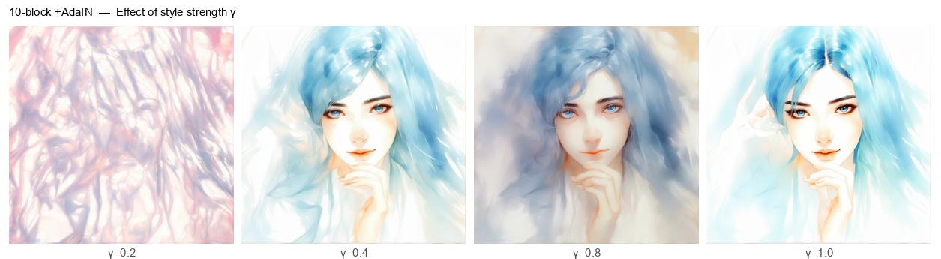
\includegraphics[width=\columnwidth]{fig_gamma_10blk.pdf}
  \caption{10块配置下不同$\gamma$值的风格迁移效果。与5块配置相比，10块在相同$\gamma$下风格注入更强，但内容细节的保持略逊于5块配置。}
  \label{fig:gamma_10blk}
\end{figure}

\subsection{块数消融实验}

为验证目标块数量对风格迁移效果的影响，在固定$\gamma=0.6$且使用AdaIN的条件下，测试1块、2块、5块配置，结果如表~\ref{tab:block_ablation}所示。

\begin{table}[htbp]
  \centering
  \caption{块数消融实验结果（固定$\gamma=0.6$，使用AdaIN）。1块配置风格注入最保守，5块配置获得最优Art-FID，2块配置结果居中。更多块带来更强风格注入，5块在效果与效率之间取得最佳平衡。}
  \label{tab:block_ablation}
  \small
  \setlength{\tabcolsep}{3pt}
  \begin{tabular}{clccc}
    \toprule
    块数 & 对应变体 & FID$\downarrow$ & Art-FID$\downarrow$ & LPIPS \\
    \midrule
    1块 & V1 (adain\_1blk)  & 73.34 & 103.17 & 0.581 \\
    2块 & V2 (adain\_2blk)  & 88.54 & 98.42  & 0.599 \\
    5块 & V7 (proc05\_adain) & 78.14 & 85.43  & 0.629 \\
    \bottomrule
  \end{tabular}
\end{table}

\textbf{结论：}更多目标块带来更强风格注入（Art-FID从103.17降至85.43），但计算开销也相应增加。5块配置在风格迁移效果和计算效率之间取得了平衡。图~\ref{fig:block_compare}直观对比了1块与5块配置在不同$\gamma$值下的生成差异。

\begin{figure}[htbp]
  \centering
  
\includegraphics[width=\columnwidth]{fig_block_compare.pdf}
  \caption{1块与5块配置在不同$\gamma$值下的风格迁移效果对比。上行为1块配置，下行为5块配置（本文方法）。更多块数带来更强的风格注入（下行风格纹理更明显），同时内容结构保持依然良好。}
  \label{fig:block_compare}
\end{figure}

\subsection{定性结果分析}

\subsubsection{不同块数与AdaIN的效果对比}

表~\ref{tab:qual_blocks}对比了四种基础配置的生成结果。图~\ref{fig:adain_compare}进一步展示了AdaIN模块在1块配置下对色彩协调性的影响。

\begin{table}[htbp]
  \centering
  \caption{不同块数与AdaIN配置的定性对比。使用AdaIN的配置色彩协调性更优、风格覆盖更均匀；不使用AdaIN的配置风格迁移更强但内容结构退化更明显。}
  \label{tab:qual_blocks}
  \small
  \setlength{\tabcolsep}{3pt}
  \begin{tabular}{lc>{\raggedright\arraybackslash}p{2.8cm}}
    \toprule
    变体 & 块数 & 观察结果 \\
    \midrule
    adain\_1blk   & 1 & 风格注入集中，纹理迁移明显 \\
    adain\_2blk   & 2 & 风格覆盖均匀，色彩更协调 \\
    no\_adain\_1blk & 1 & 风格迁移较强，内容保留略逊 \\
    no\_adain\_2blk & 2 & 风格注入增强，结构更模糊 \\
    \bottomrule
  \end{tabular}
\end{table}

\begin{figure}[htbp]
  \centering
  
\includegraphics[width=\columnwidth]{fig_adain_compare.pdf}
  \caption{AdaIN模块对风格迁移效果的影响（1块配置）。上行为使用AdaIN的生成结果，下行为不使用AdaIN的结果。AdaIN模块显著提升了色彩协调性与整体氛围一致性，尤其在高$\gamma$值时差异更为明显。}
  \label{fig:adain_compare}
\end{figure}

\subsubsection{不同Gamma值的效果对比}

不同$\gamma$值下的生成效果：$\gamma = 0.0$时内容占主导，风格仅在最强烈纹理区域体现；$\gamma = 0.2$时风格开始显现但以内容为主；$\gamma = 0.6$为最佳平衡点，内容结构良好保持，风格纹理和色彩成功迁移；$\gamma = 0.8$时风格占据主导，内容细节开始丢失；$\gamma = 1.0$时完全风格化，空间布局虽保留但细粒度语义已丢失。

\subsubsection{用户偏好研究}

除了定量指标外，我们还进行了用户偏好研究。7名参与者对7种方法在7组不同的内容-风格对上的生成结果进行了排序（1为最佳，7为最差）。尽管样本量有限，结果仍提供了有参考价值的定性趋势：如图~\ref{fig:user_study}所示，我们的完整方法（V7, $\gamma = 0.6$）在多数配对中获得最高排名，特别是在配对\#1、\#4和\#7中表现优异。未来工作将扩大用户研究规模以获取统计显著性。

\begin{figure}[htbp]
  \centering
  
\includegraphics[width=\columnwidth]{image4.pdf}
  \caption{用户偏好研究结果：7名参与者对7种方法在7组内容-风格对上的排序评分（1为最佳，7为最差）。}
  \label{fig:user_study}
\end{figure}

\begin{figure*}[tbp]
  \centering
  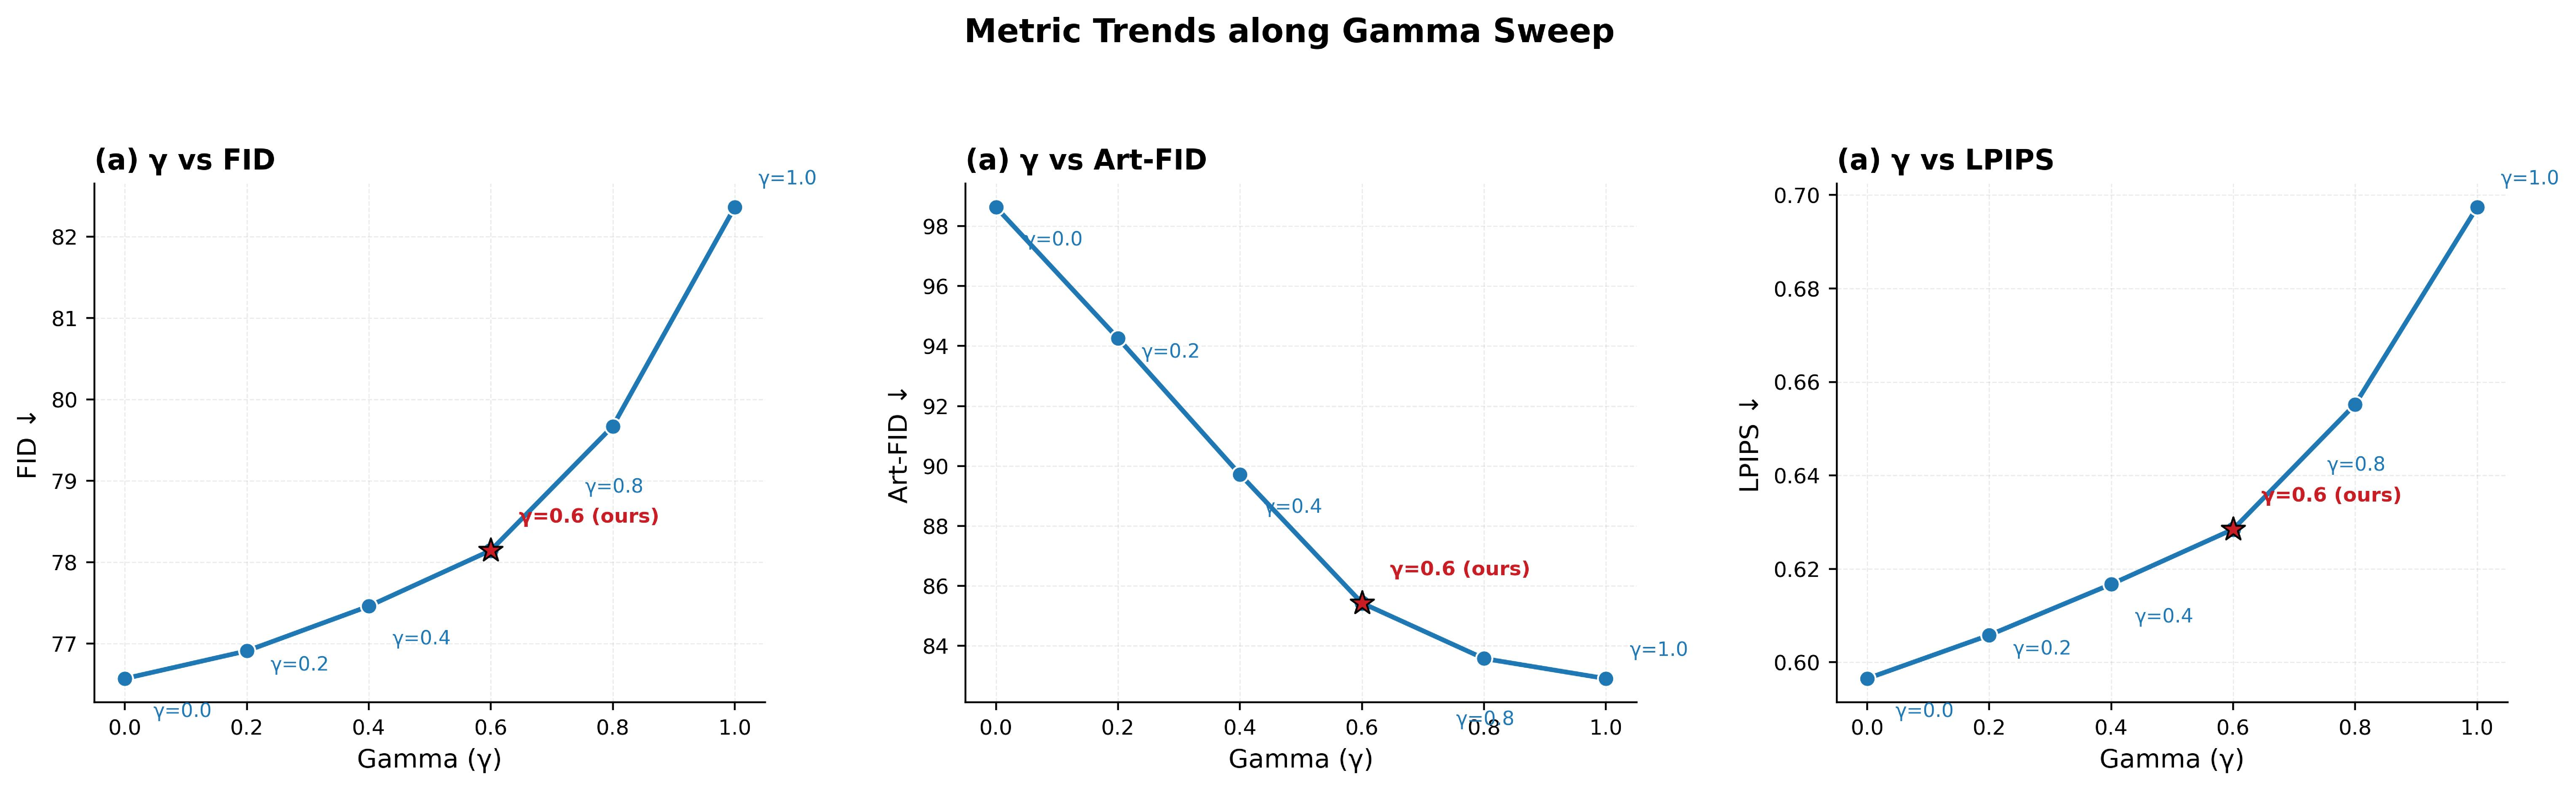
\includegraphics[width=\textwidth]{fig_ref_comprehensive.pdf}
  \caption{不同配置下的风格迁移效果综合对比。涵盖不同块数（1块、2块、5块）、不同$\gamma$值（0.2--1.0）以及AdaIN开关条件下的生成效果，系统展示了各参数对风格迁移结果的影响规律。}
  \label{fig:comprehensive}
\end{figure*}

图~\ref{fig:gallery}（文首效果展示）以三组不同内容-风格配对的完整对比呈现了本文方法的整体迁移效果。图~\ref{fig:comprehensive}则系统性地展示了不同块数、$\gamma$值和AdaIN开关配置下的综合生成效果：块数的增加有效增强了风格注入强度，$\gamma$值的升高使风格纹理逐步占据主导，而AdaIN模块的使用则在色彩和谐性与风格覆盖均匀性方面带来了显著提升。

\subsubsection{提示词的影响}

我们观察到提示词质量对生成结果有显著影响。使用简单提示词时，模型对内容理解有限，细节匮乏；使用详细提示词时，模型能更准确理解用户意图，风格一致性和视觉质量显著提升。这表明在风格迁移任务中，文本提示是引导扩散模型理解内容语义的关键因素。

\subsection{实验中的关键发现}

\subsubsection{Canny边缘图分辨率与推理时间的权衡}

Canny边缘图的精细程度直接影响生成效果和推理效率。表~\ref{tab:resolution_canny}和表~\ref{tab:resolution_input}测试了不同分辨率下的推理时间。

\begin{table}[htbp]
  \centering
  \caption{Canny分辨率与推理时间对比。高分辨率Canny边缘图可提供更丰富的结构信息从而提升生成效果，但推理时间呈非线性增长，且精细边缘图可能引入额外的人工痕迹。}
  \label{tab:resolution_canny}
  \small
  \begin{tabular}{lll}
    \toprule
    输入分辨率 & Canny分辨率 & 推理时间 \\
    \midrule
    1080$\times$599   & 1080$\times$599   & 约12秒 \\
    5774$\times$1536  & 5774$\times$1536  & 约68秒 \\
    \bottomrule
  \end{tabular}
\end{table}

\begin{table}[htbp]
  \centering
  \caption{输入分辨率与推理时间对比。推理时间随分辨率增长呈非线性增长。合适的Canny分辨率需在图像质量与计算开销之间权衡：过低会丢失主体细节，过高则耗时剧增。}
  \label{tab:resolution_input}
  \small
  \begin{tabular}{lll}
    \toprule
    输入分辨率 & 推理时间 & 说明 \\
    \midrule
    1080$\times$1050  & 约13秒   & 标准分辨率 \\
    2106$\times$2048  & 约63秒 & 高分辨率 \\
    \bottomrule
  \end{tabular}
\end{table}

\begin{figure}[htbp]
  \centering
  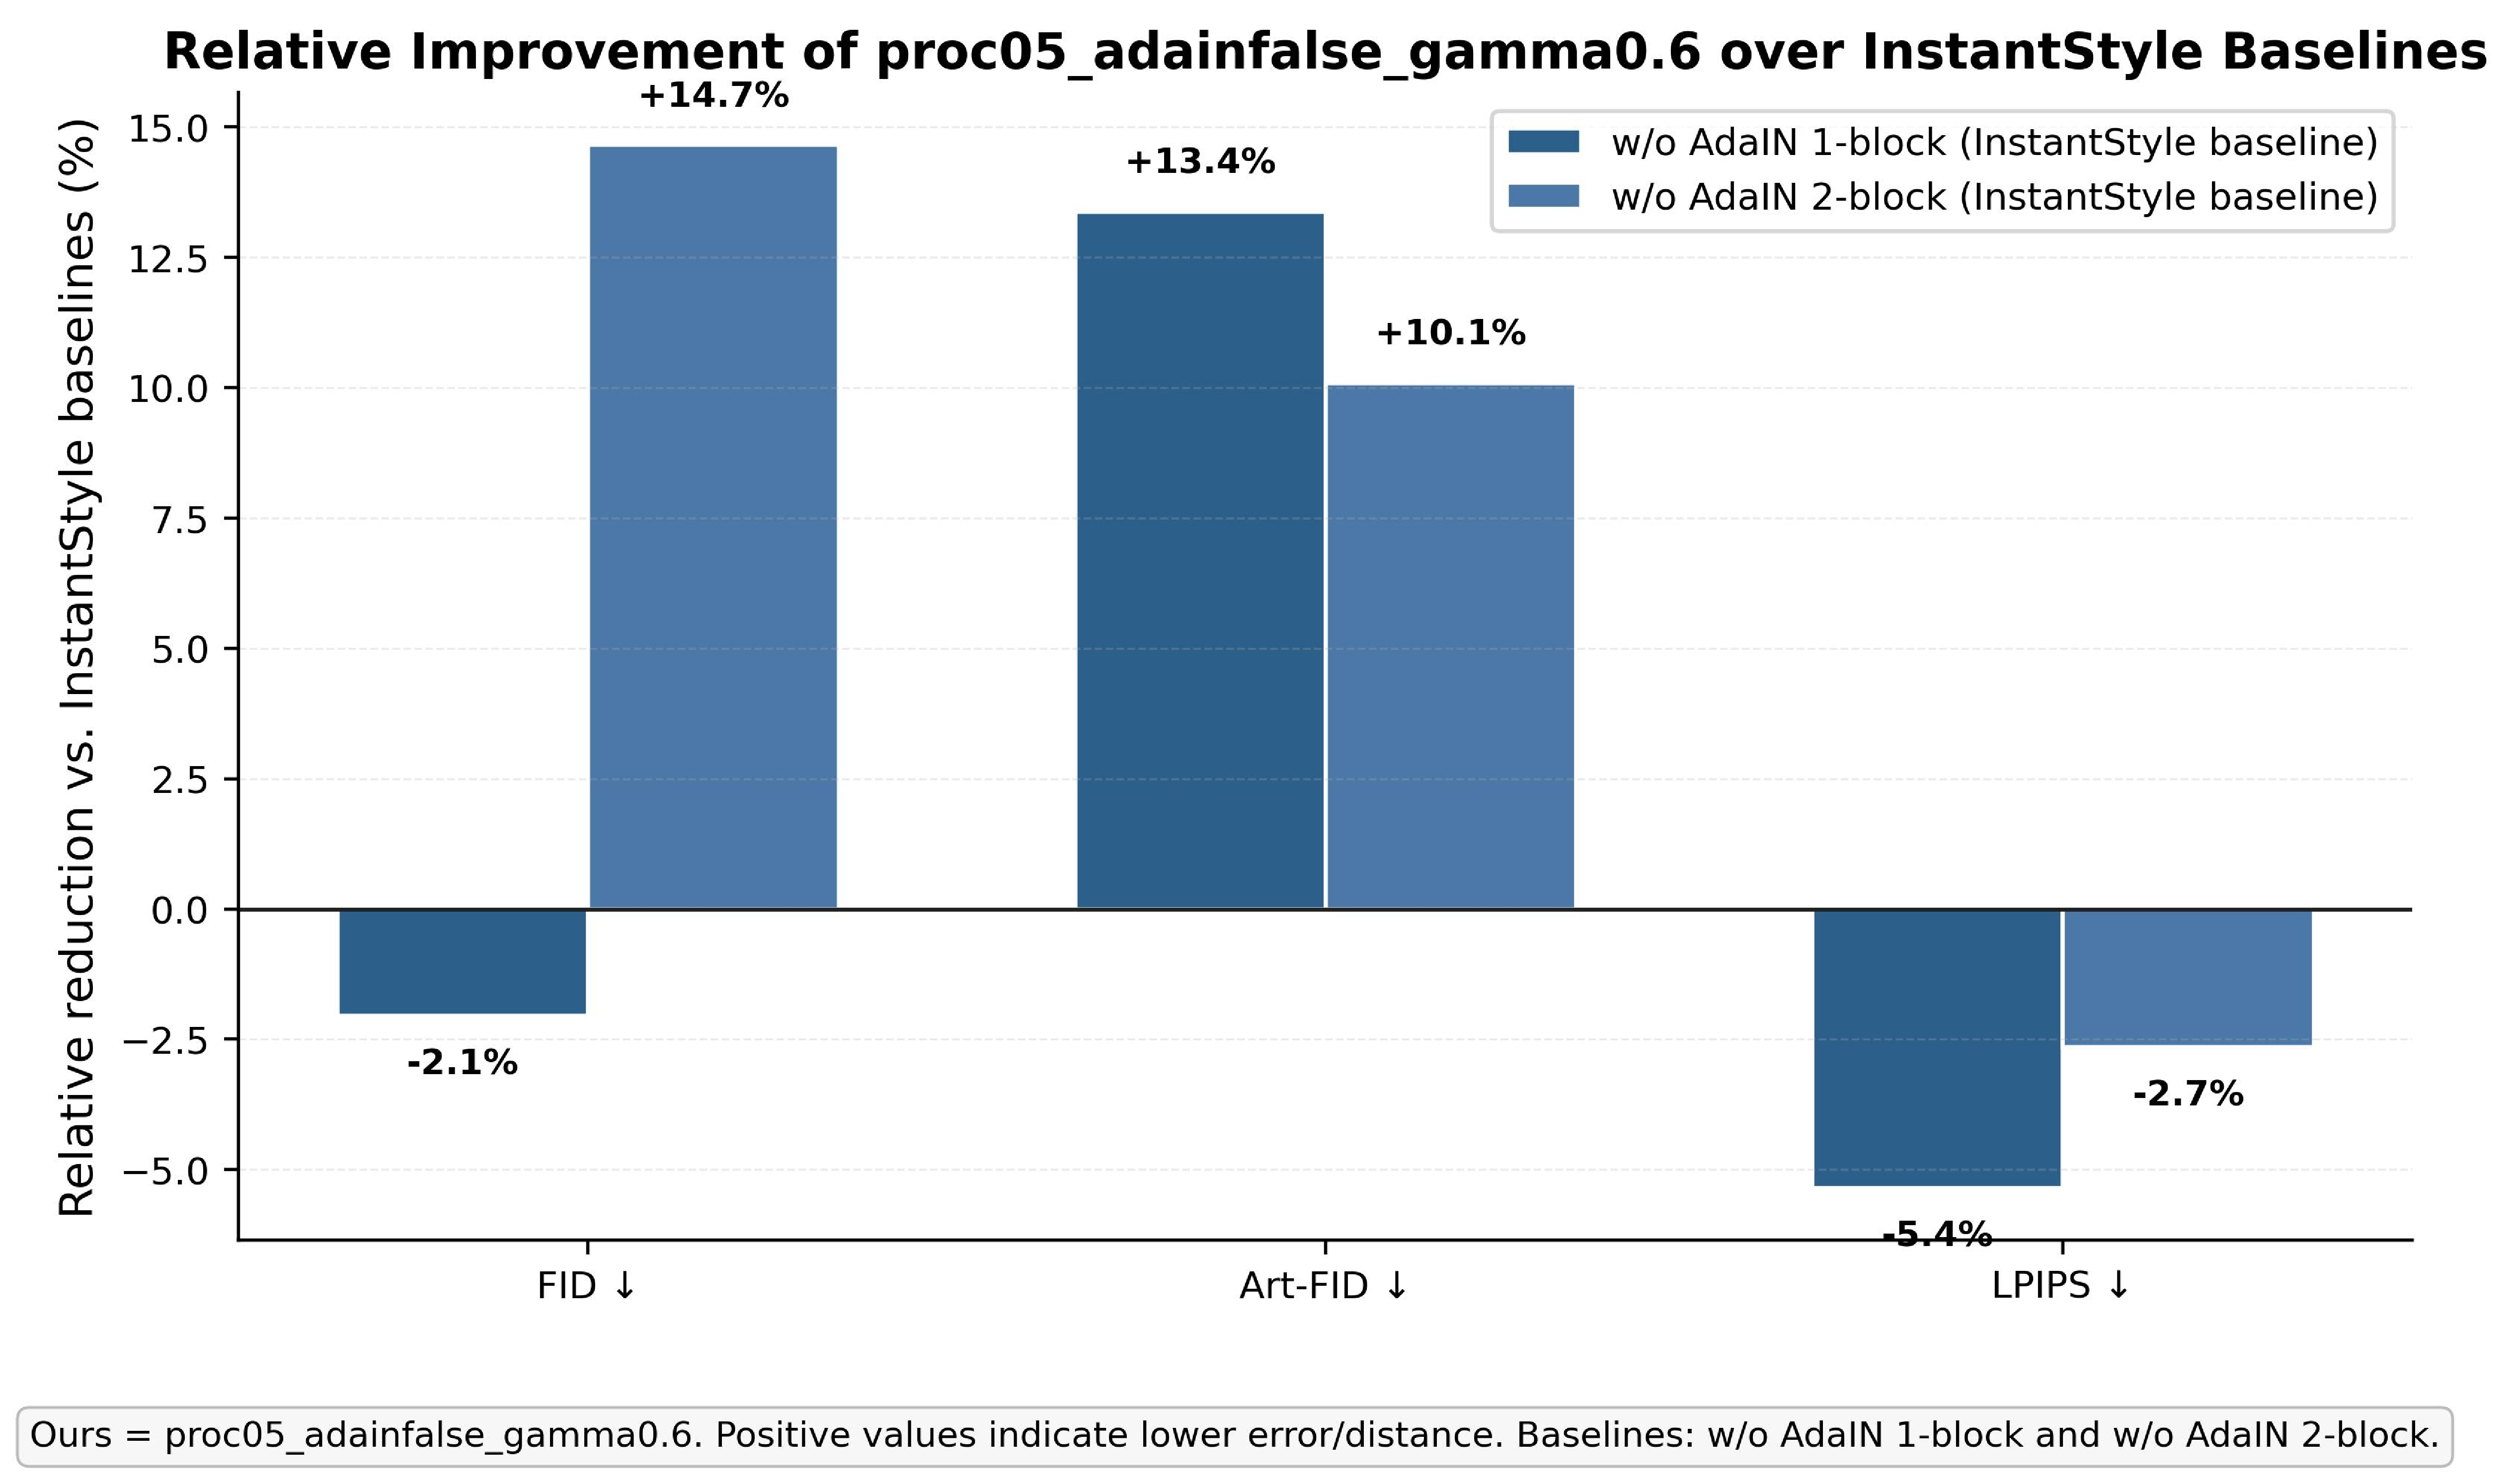
\includegraphics[width=\columnwidth]{fig_canny_res.pdf}
  \caption{不同分辨率下的Canny边缘检测效果对比。高分辨率（下）能够保留更精细的边缘细节，但推理时间显著增加（约68秒 vs 约12秒），且可能引入额外的人工痕迹。}
  \label{fig:canny_res}
\end{figure}

\begin{figure*}[ht]
  \centering
  
\includegraphics[width=\textwidth]{fig_input_res.pdf}
  \caption{不同输入分辨率下的风格迁移效果对比。高分辨率输入可提供更多细节信息，但推理时间随分辨率呈非线性增长，需在实际应用中权衡。}
  \label{fig:input_res}
\end{figure*}

\textbf{关键发现：}(1) 更精细的Canny边缘图能提升生成效果，模型获得更丰富的结构信息；(2) 但精细边缘图也可能引入额外的人工痕迹——模型可能生成边缘图中不存在但统计上合理的细节；(3) 推理时间随分辨率呈非线性增长；(4) 需在过于精细（人工痕迹多、开销大）和过于粗糙（丢失细节）之间找平衡。如图~\ref{fig:canny_res}所示，不同分辨率下Canny边缘检测的精细程度差异显著；图~\ref{fig:input_res}则对比了不同输入分辨率下的风格迁移效果。基于这些观察，前端支持用户动态调节Canny边缘检测参数。

\subsubsection{设备资源限制}

扩散模型（Stable Diffusion基础模型约7--8GB，加上VAE、ControlNet、IP-Adapter等模块，总显存需求约15--20GB）在消费级GPU上运行仍有一定挑战。即使使用V100-32GB，批量生成时也面临显存压力和GPU资源竞争等问题。我们的方法通过选择性块注入（仅5块）有效减少了计算开销，使整个流程在V100上能够流畅运行。

%% ================================================
%% 5. 交互式前端
%% ================================================
\section{交互式前端}

为提升实际可用性和用户体验，我们基于Gradio框架构建了名为\textbf{InstantStyle Control Studio}的交互式前端。

\subsection{前端功能模块}

{\bfseries (1) 图像输入模块：}内容图像上传、风格图像上传、自动生成并预览Canny边缘图。

{\bfseries (2) 提示词控制模块：}正向提示词（描述期望生成结果）、反向提示词（不希望出现的元素），支持长文本输入。

{\bfseries (3) ControlNet/Canny参数调节：}Canny Low/High Threshold（边缘检测灵敏度）、Conditioning Scale（ControlNet控制强度）、Bilateral Filter参数（边缘预处理去噪）。

{\bfseries (4) AdaIN风格融合模块：}AdaIN Alpha（融合强度）、AdaIN Beta（融合偏置），支持实时预览。

{\bfseries (5) 生成参数控制：}Steps（DDIM采样步数，默认50）、CFG Scale（无分类器引导，默认7.5）、Seed（随机种子）、IP-Adapter风格强度。

{\bfseries (6) 输出管理：}输出目录设置、生成状态实时显示、结果画廊展示。

\subsection{前端特性与价值}

前端支持参数热重载（调整参数后无需重启即可查看效果）、Canny边缘图实时预览、配置保存为JSON文件、批量生成。设计目标是降低使用门槛，使非专业用户也能通过直观的滑块、开关和预览图理解各参数对生成结果的影响。图~\ref{fig:gradio}展示了该前端的整体界面布局。

\begin{figure}[htbp]
  \centering
  
\includegraphics[width=\columnwidth]{fig_gradio.pdf}
  \caption{InstantStyle Control Studio交互式前端界面。用户可通过左侧面板上传内容与风格图像、调节ControlNet/Canny参数、设置AdaIN融合系数及生成参数；右侧区域实时展示Canny边缘图预览与风格化输出结果。}
  \label{fig:gradio}
\end{figure}

%% ================================================
%% 6. 未来工作
%% ================================================
\section{未来工作}

\subsection{与现有方法的定量比较}
当前实验聚焦于自身消融研究以验证各组件有效性，尚未与InST[12]、StyleDiffusion[13]、InstantStyle[17]等方法进行同等条件下的定量比较。计划在统一的数据集和评估协议下进行系统性的方法间对比。

\subsection{自适应Canny边缘图生成}
当前需手动调节Canny阈值，且最优值因图像内容而异。计划引入HED、RINDNet等更优边缘提取模型，实现自适应边缘图生成，减少手动调参需求。

\subsection{VLM提示词自动生成}
当前提示词需人工编写或借助外部模型生成。计划引入开源视觉语言模型（如Qwen-VLM、LLaVA）自动为风格图像生成高质量提示词，降低使用门槛。

\subsection{扩展至SDXL架构}
计划将KV融合方法适配到SDXL架构，重新识别有效块并调整融合策略，利用SDXL更强大的生成能力提升风格迁移质量。

\subsection{引入Tile ControlNet}
高分辨率Canny边缘图可能引入人工痕迹。计划使用Tile ControlNet通过分块处理缓解高分辨率下的人工痕迹问题，同时保持细节丰富度。

\subsection{全块级贡献度分析}
当前仅测试1块、2块、5块配置。计划逐个测试U-Net各块的风格迁移贡献度，建立块-风格映射关系，为方法优化提供理论依据。

\subsection{多条件ControlNet融合}
当前仅集成Canny ControlNet。计划探索多个ControlNet（边缘+深度+姿态等）的协同工作，进一步提升内容保持能力。

%% ================================================
%% 7. 结论与局限性
%% ================================================
\FloatBarrier
\section{结论与局限性}

\subsection{结论}

本文提出了一种无需训练的AdaIN StyleKV风格迁移方法。主要贡献包括：

\begin{itemize}
  \setlength{\itemsep}{0pt}
\item {\bfseries 方法创新：}提出风格图像KV与内容图像KV的加权融合策略，实现自注意力层特征的精确操控；将AdaIN引入初始潜空间，通过调整初始噪声的通道统计量改善色彩协调性。
\item {\bfseries 系统验证：}在COCO+WikiArt数据集上构建7组方法变体，生成5000张图像进行系统消融实验。实验表明完整方法在风格保真度与内容保留之间实现了较优平衡。
\item {\bfseries 实践价值：}基于Gradio构建交互式前端，支持Canny调节、AdaIN参数控制、实时对比等功能。
\item {\bfseries 经验总结：}详细记录了实验中的关键发现，包括提示词质量的重要性、Canny分辨率与推理时间的权衡等。
\end{itemize}

\subsection{局限性}

尽管本文方法取得了较好效果，仍存在以下局限性，如表~\ref{tab:limitations}所示。这些局限性同时也是第6节未来工作的重点攻关内容。

\begin{table}[htbp]
  \centering
  \caption{本文方法的主要局限性及对应改进方向。}
  \label{tab:limitations}
  \small
  \setlength{\tabcolsep}{3pt}
  \begin{tabular}{p{2.2cm}p{3.2cm}p{2.2cm}}
    \toprule
    局限性 & 说明 & 对应改进方向 \\
    \midrule
    缺乏外部方法对比 & 仅进行消融实验，未与InST等方法直接比较 & 统一基准下的系统对比 \\
    全块级消融缺失 & 仅测试1、2、5块，未系统验证所有块 & 全块级贡献度分析 \\
    ControlNet单一 & 仅测试Canny，其他条件未集成 & 多条件ControlNet融合 \\
    提示词依赖外部 & 依赖外部模型生成，未集成开源VLM & VLM提示词自动生成 \\
    设备资源受限 & 需V100级别GPU，消费级设备难以运行 & 模型轻量化探索 \\
    数据集规模有限 & COCO(20张)+WikiArt(40张) & 更大规模数据集验证 \\
    \bottomrule
  \end{tabular}
\end{table}

\subsection{未来展望}

风格迁移是一个充满活力的研究领域，随着扩散模型的不断发展，以下方向值得持续关注：(1) 免训练方法的进一步优化，在保持内容结构的同时实现更精确的风格控制；(2) 多模态风格的融合，结合文本描述、参考图像、色彩调色板等多种条件；(3) 风格迁移的可解释性，理解U-Net各层在风格迁移中的角色；(4) 轻量化部署，将方法压缩并部署到移动端。

%% ================================================
%% 致谢
%% ================================================
\section*{致谢}
感谢所有对本文工作提供支持和帮助的老师和同学。感谢AutoDL平台提供的GPU计算资源支持。感谢开源社区贡献的Stable Diffusion、ControlNet、IP-Adapter等优秀工作，为本文的研究提供了坚实的基础。此外，感谢参与用户偏好研究的 7 位匿名志愿者，他们的反馈为本文的定性分析提供了有价值的参考。

%% ================================================
%% 参考文献
%% ================================================
\begin{thebibliography}{99}

\bibitem{efros1999} A.~A.~Efros and T.~K.~Leung, ``Texture synthesis by non-parametric sampling,'' in \emph{Proc. ICCV}, 1999.

\bibitem{gatys2016} L.~A.~Gatys, A.~S.~Ecker, and M.~Bethge, ``Image style transfer using convolutional neural networks,'' in \emph{Proc. CVPR}, 2016.

\bibitem{ulyanov2016} D.~Ulyanov, V.~Lebedev, A.~Vedaldi, and V.~Lempitsky, ``Texture networks: Feed-forward synthesis of textures and stylized images,'' in \emph{Proc. ICML}, 2016.

\bibitem{huang2017} X.~Huang and S.~Belongie, ``Arbitrary style transfer in real-time with adaptive instance normalization,'' in \emph{Proc. ICCV}, 2017.

\bibitem{zhu2017} J.-Y.~Zhu, T.~Park, P.~Isola, and A.~A.~Efros, ``Unpaired image-to-image translation using cycle-consistent adversarial networks,'' in \emph{Proc. ICCV}, 2017.

\bibitem{choi2018} Y.~Choi, M.~Choi, M.~Kim, J.-W.~Ha, S.~Kim, and J.~Choo, ``StarGAN: Unified generative adversarial networks for multi-domain image-to-image translation,'' in \emph{Proc. CVPR}, 2018.

\bibitem{karras2019} T.~Karras, S.~Laine, and T.~Aila, ``A style-based generator architecture for generative adversarial networks,'' in \emph{Proc. CVPR}, 2019.

\bibitem{sohl2015} J.~Sohl-Dickstein, E.~A.~Weiss, N.~Maheswaranathan, and S.~Ganguli, ``Deep unsupervised learning using nonequilibrium thermodynamics,'' in \emph{Proc. ICML}, 2015.

\bibitem{ho2020} J.~Ho, A.~Jain, and P.~Abbeel, ``Denoising diffusion probabilistic models,'' in \emph{Proc. NeurIPS}, 2020.

\bibitem{song2020} Y.~Song and S.~Ermon, ``Improved techniques for training score-based generative models,'' in \emph{Proc. NeurIPS}, 2020.

\bibitem{rombach2022} R.~Rombach, A.~Blattmann, D.~Lorenz, P.~Esser, and B.~Ommer, ``High-resolution image synthesis with latent diffusion models,'' in \emph{Proc. CVPR}, 2022.

\bibitem{zhang2023inst} Y.~Zhang, N.~Huang, F.~Tang, H.~Huang, C.~Ma, W.~Dong, and C.~Xu, ``InST: Inversion-based style transfer with diffusion models,'' in \emph{Proc. CVPR}, 2023.

\bibitem{wang2023style} Z.~Wang, L.~Zhao, W.~Xing, and D.~Lu, ``StyleDiffusion: Controllable disentangled style transfer via diffusion models,'' in \emph{Proc. ICCV}, 2023.

\bibitem{jeong2023} J.~Jeong, M.~Kwon, and Y.~Uh, ``DiffStyle: Training-free style transfer with diffusion models,'' \emph{arXiv preprint arXiv:2312.01714}, 2023.

\bibitem{zhang2023controlnet} L.~Zhang, A.~Rao, and M.~Agrawala, ``Adding conditional control to text-to-image diffusion models,'' in \emph{Proc. ICCV}, 2023.

\bibitem{hertz2023} A.~Hertz, R.~Mokady, J.~Tenenbaum, K.~Aberman, Y.~Pritch, and D.~Cohen-Or, ``Style Injection: Training-free style transfer using self-attention,'' \emph{arXiv preprint arXiv:2312.08008}, 2023.

\bibitem{wang2024instantstyle} H.~Wang, Q.~Wang, X.~Bai, Z.~Qin, and A.~Chen, ``InstantStyle: Free lunch towards style-preserving in text-to-image generation,'' \emph{arXiv preprint arXiv:2404.02733}, 2024.

\bibitem{lin2014} T.-Y.~Lin, M.~Maire, S.~Belongie, J.~Hays, P.~Perona, D.~Ramanan, P.~Doll\'{a}r, and C.~L.~Zitnick, ``Microsoft COCO: Common objects in context,'' in \emph{Proc. ECCV}, 2014.

\bibitem{wikiart} WikiArt, ``WikiArt Visual Art Encyclopedia.'' [Online]. Available: \url{https://www.wikiart.org/}.

\bibitem{artfid} M.~Wright and B.~Ommer, ``Art-FID: Quantitative evaluation of neural style transfer,'' in \emph{Proc. GCPR}, 2022.

\bibitem{heusel2017} M.~Heusel, H.~Ramsauer, T.~Unterthiner, B.~Nessler, and S.~Hochreiter, ``GANs trained by a two time-scale update rule converge to a local Nash equilibrium,'' in \emph{Proc. NeurIPS}, 2017.

\bibitem{zhang2018lpips} R.~Zhang, P.~Isola, A.~A.~Efros, E.~Shechtman, and O.~Wang, ``The unreasonable effectiveness of deep features as a perceptual metric,'' in \emph{Proc. CVPR}, 2018.

\bibitem{simonyan2015} K.~Simonyan and A.~Zisserman, ``Very deep convolutional networks for large-scale image recognition,'' in \emph{Proc. ICLR}, 2015.

\bibitem{johnson2016} J.~Johnson, A.~Alahi, and L.~Fei-Fei, ``Perceptual losses for real-time style transfer and super-resolution,'' in \emph{Proc. ECCV}, 2016.

\bibitem{park2019} D.~Y.~Park and K.~H.~Lee, ``Arbitrary style transfer with style-attentional networks,'' in \emph{Proc. CVPR}, 2019.

\bibitem{deng2022} Y.~Deng, F.~Tang, W.~Dong, C.~Ma, X.~Pan, L.~Wang, and C.~Xu, ``StyTr$^2$: Image style transfer with transformers,'' in \emph{Proc. CVPR}, 2022.

\bibitem{an2021} J.~An, S.~Huang, Y.~Song, D.~Dou, W.~Liu, and J.~Luo, ``ArtFlow: Unbiased image style transfer via reversible neural flows,'' in \emph{Proc. CVPR}, 2021.

\bibitem{liu2021} S.~Liu, T.~Lin, D.~He, F.~Li, M.~Wang, X.~Li, Z.~Sun, Q.~Li, and E.~Ding, ``AdaAttN: Revisit attention mechanism in arbitrary neural style transfer,'' in \emph{Proc. ICCV}, 2021.

\bibitem{chen2021} H.~Chen, L.~Zhao, Z.~Wang, H.~Zhang, Z.~Zuo, A.~Li, W.~Xing, and D.~Lu, ``DualAST: Dual style-learning networks for artistic style transfer,'' in \emph{Proc. CVPR}, 2021.

\bibitem{karras2020} T.~Karras, S.~Laine, M.~Aittala, J.~Hellsten, J.~Lehtinen, and T.~Aila, ``Analyzing and improving the image quality of StyleGAN,'' in \emph{Proc. CVPR}, 2020.

\bibitem{karras2021} T.~Karras, M.~Aittala, S.~Laine, E.~H\"{a}rk\"{o}nen, J.~Hellsten, J.~Lehtinen, and T.~Aila, ``Alias-free generative adversarial networks,'' in \emph{Proc. NeurIPS}, 2021.

\end{thebibliography}

%% ================================================
%% 附录
%% ================================================
\FloatBarrier
\section*{附录}

\subsection*{A. 7组变体完整数据}

表~\ref{tab:appendix_a}列出了7组变体的完整实验数据，与正文表3一致。

\begin{table}[htbp]
  \centering
  \small
  \caption{7组变体完整定量数据（与正文表3一致）。}
  \label{tab:appendix_a}
  \begin{tabular}{lccc}
    \toprule
    变体名称 & FID$\downarrow$ & Art-FID$\downarrow$ & LPIPS \\
    \midrule
    V1 (adain\_1blk)       & 73.34 & 103.17 & 0.581 \\
    V2 (adain\_2blk)       & 88.54 & 98.42  & 0.599 \\
    V3 (no\_adain\_1blk)   & 76.57 & 98.63  & 0.597 \\
    V4 (no\_adain\_2blk)   & 91.56 & 95.02  & 0.612 \\
    V5 (adain\_no\_ctrl)   & 70.75 & 104.12 & 0.746 \\
    V6 (proc05\_no\_adain) & 78.48 & 90.76  & 0.599 \\
    V7 (proc05\_adain)     & 78.14 & 85.43  & 0.629 \\
    \bottomrule
  \end{tabular}
\end{table}

\subsection*{B. Gamma消融实验数据}

表~\ref{tab:appendix_b}列出了$\gamma$消融实验的完整数据。

\begin{table}[htbp]
  \centering
  \small
  \caption{$\gamma$消融实验完整数据（5块+AdaIN+ControlNet，与正文表4一致）。}
  \label{tab:appendix_b}
  \begin{tabular}{cccc}
    \toprule
    $\gamma$ & FID$\downarrow$ & Art-FID$\downarrow$ & LPIPS \\
    \midrule
    0.0 & 76.57 & 98.63 & 0.597 \\
    0.2 & 76.91 & 94.26 & 0.606 \\
    0.4 & 77.46 & 89.72 & 0.617 \\
    0.6 & 78.14 & 85.43 & 0.629 \\
    0.8 & 79.67 & 83.58 & 0.655 \\
    1.0 & 82.36 & 82.91 & 0.697 \\
    \bottomrule
  \end{tabular}
\end{table}

\subsection*{C. 块数消融实验数据}

表~\ref{tab:appendix_c}列出了块数消融实验的完整数据。

\begin{table}[htbp]
  \centering
  \small
  \caption{块数消融实验完整数据（$\gamma = 0.6$，使用AdaIN，与正文表5一致）。}
  \label{tab:appendix_c}
  \begin{tabular}{clccc}
    \toprule
    块数 & 对应变体 & FID$\downarrow$ & Art-FID$\downarrow$ & LPIPS \\
    \midrule
    1块 & V1 (adain\_1blk)  & 73.34 & 103.17 & 0.581 \\
    2块 & V2 (adain\_2blk)  & 88.54 & 98.42  & 0.599 \\
    5块 & V7 (proc05\_adain) & 78.14 & 85.43  & 0.629 \\
    \bottomrule
  \end{tabular}
\end{table}

\end{document}
